\section{Neural Networks}\label{sec:nnets}
Neural networks are biologically inspired classifiers which is why they are often called "artificial neural networks" to distinguish them from the organic kind. However, in reality human neural networks are so much more capable and complex from artificial neural networks that it is usually better to not draw too many parallels between the two.\\
\textbf{The need for non-linear classifiers: }\\
\begin{figure}[H]%
    \center%
    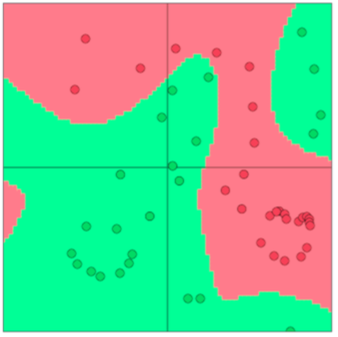
\includegraphics[width=0.5\textwidth]{images/eman/NonlinearBoundary.png}%
     % you need to add the caption for the list of figures
\caption[Nonlinear Boundary Using Neural Network]{We see here how a non-linear decision boundary separates the data very well. This is the prowess of neural networks.}\label{fig:NonlinearBoundary}%
  \end{figure}
since most data are not linearly separable and thus, our classification performance on them is limited. Neural networks are a family of classifiers with non-linear decision boundary as seen in Figure~\ref{fig:NonlinearBoundary}. Now that we know the sort of decision boundaries neural networks create, let us see how they manage doing so.
\subsection{A Neuron}\label{sec:neuron}
A neuron is the fundamental building block of neural networks. We will see that a neuron can be one of many functions that allows for non-linearities to accrue in the network.\\
A neuron is a generic computational unit that takes $n$ inputs and produces a single output. What differentiates the outputs of different neurons is their parameters (also referred to as their weights). One of the most popular choices for neurons is the "sigmoid" or "binary logistic regression" unit. This unit takes an $n$-dimensional input vector $x$ and produces the scalar activation (output) $a$. This neuron is also associated with an $n$-dimensional weight vector, $w$, and a bias scalar, $b$. The output of this neuron is then:
$$ a = \frac{1}{1 + \exp(-(w^Tx + b))}$$
We can also combine the weights and bias term above to equivalently formulate:
$$ a = \frac{1}{1 + \exp(-[w^T~~~b] \cdot[x~~~1])}$$
This formulation can be visualized in the manner shown in Figure~\ref{fig:sigmoidneuron}.
\begin{figure}[H]%
    \center%
    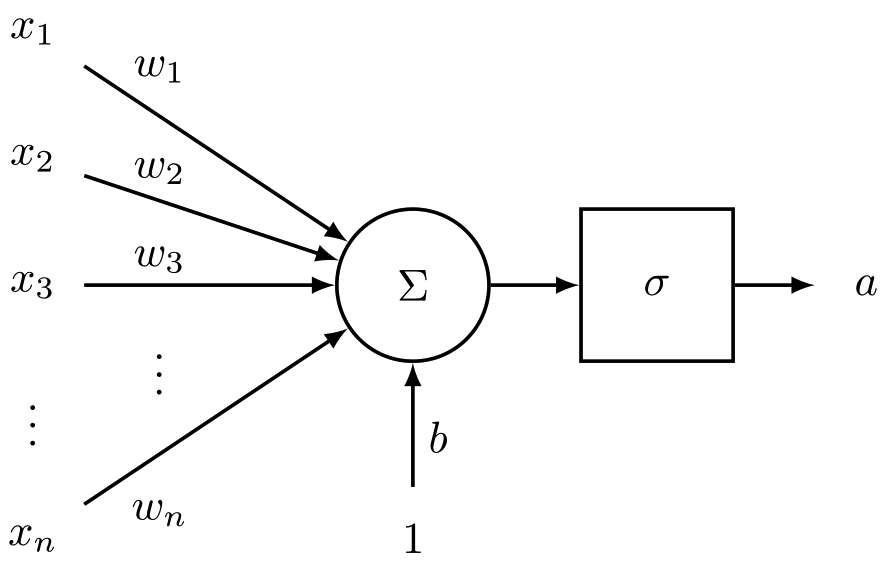
\includegraphics[width=0.5\textwidth]{images/eman/sigmoidneuron.png}%
     % you need to add the caption for the list of figures
\caption[Sigmoid neuron in neural network]{This image captures how in a sigmoid neuron, the input vector $x$ is first scaled, summed, added to a bias unit, and then passed to the squashing sigmoid function.}\label{fig:sigmoidneuron}%
  \end{figure}
\subsection{A Single Layer of Neurons}\label{sec:neuronlayer}
We extend the idea above to multiple neurons by considering the case where the input $x$ is fed as an input to multiple such neurons as shown in Figure~\ref{fig:SingleLayerNeuralNetwork}.
\begin{figure}[H]%
    \center%
    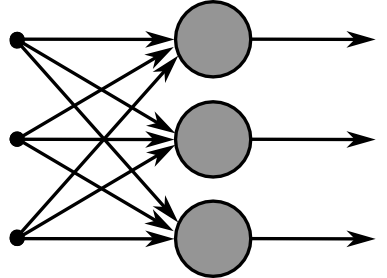
\includegraphics[width=0.5\textwidth]{images/eman/SingleLayerNeuralNetwork.png}%
     % you need to add the caption for the list of figures
\caption[Single Layer Neural Network]{This image captures how multiple sigmoid units are stacked on the right, all of which receive the same input $x$.}\label{fig:SingleLayerNeuralNetwork}%
  \end{figure}
If we refer to the different neurons' weights as $\{w^{(1)}, \cdots, w^{(m)}\}$ and the biases as $\{b_1, \cdots, b_m\}$, we can say the respective activations are  $\{a_1, \cdots, a_m\}$:
\begin{align*}
a_1 &= \frac{1}{1 + \exp(w^{(1)T}x + b_1)}\\
\vdots \\
a_m &= \frac{1}{1 + \exp(w^{(m)T}x + b_m)}
\end{align*}
\subsection{Feed-forward Neural Network}
A feedforward neural network is an artificial neural network wherein connections between the nodes do not form a cycle. As such, it is different from recurrent neural networks.\\
The feedforward neural network was the first and simplest type of artificial neural network devised. In this network, the information moves in only one direction, forward, from the input nodes, through the hidden nodes (if any) and to the output nodes as shown in Figure~\ref{fig:SingleLayerNeuralNetwork}. There are no cycles or loops in the network.
\begin{figure}[H]%
    \center%
    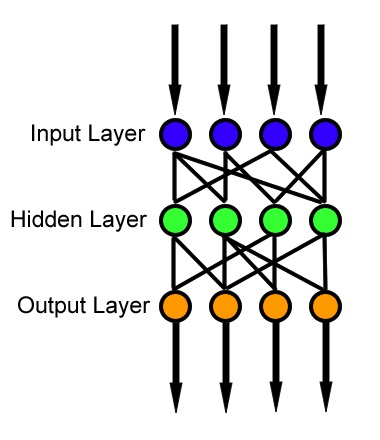
\includegraphics[width=0.5\textwidth]{images/eman/Feed_forward_neural_net.jpg}%
     % you need to add the caption for the list of figures
\caption[Feed forward Neural Network]{In a feed forward network information always moves one direction; it never goes backwards.}\label{fig:Feed_forward_neural_net}%
  \end{figure}
\subsubsection{Feed-forward Computation}\label{sec:ff}
\textbf{Dimensions for a single hidden layer neural network:}
If we represent each word using a $4$-dimensional word vector and we use a $5$-word window as input, then the input $x \in {\textbf{R}}^{20}$. If we use $8$ sigmoid units in the hidden layer and generate $1$ score output from the activations, then $W \in {\textbf{R}}^{8\times 20}$, $b \in {R}^{8}$, $U \in {R}^{8\times 1}$, $s \in {R}$.  The stage-wise feed-forward computation is then:\\
$$z = Wx + b$$
$$a = \sigma(z)$$
$$s = U^Ta$$
So far we have seen how an input vector $x \in {\textbf{R}}^n$ can be fed to a layer of sigmoid units to create activations $a \in {\textbf{R}}^m$. But what is the intuition behind doing so? Let us consider the following named-entity recognition (NER) problem in NLP as an example:

\begin{center}
\textit{"Museums in Paris are amazing"}
\end{center}
Here, we want to classify whether or not the center word \textit{"Paris"} is a named-entity. In such cases, it is very likely that we would not just want to capture the presence of words in the window of word vectors but some other interactions between the words in order to make the classification. For instance, maybe it should matter that \textit{"Museums"} is the first word only if \textit{"in"} is the second word. Such non-linear decisions can often not be captured by inputs fed directly to a Softmax function but instead require the scoring of the intermediate layer discussed in Section~\ref{sec:neuronlayer}. We can thus use another matrix $U \in R^{m\times 1}$ to generate an unnormalized score for a classification task from the activations:
$$s = U^Ta = U^T f(Wx + b)$$
where $f$ is the activation function.
\textbf{Analysis of Dimensions: }If we represent each word using a $4$-dimensional word vector and we use a $5$-word window as input (as in the above example), then the input $x \in {\textbf{R}}^{20}$. If we use $8$ sigmoid units in the hidden layer and generate $1$ score output from the activations, then $W \in {\textbf{R}}^{8\times 20}$, $b \in {\textbf{R}}^{8}$, $U \in {\textbf{R}}^{8\times 1}$, $s \in {\textbf{R}}$.

\begin{figure}[H]%
    \center%
    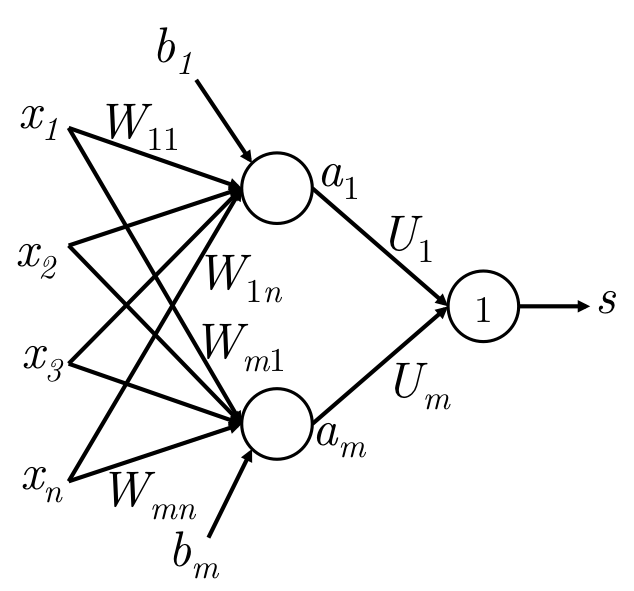
\includegraphics[width=0.5\textwidth]{images/eman/SimpleFF.png}%
     % you need to add the caption for the list of figures
\caption[Simple feed-forward network]{This image captures how a simple feed-forward network might compute its output.}\label{fig:SimpleFF}%
  \end{figure}

\subsection{Maximum Margin Objective Function}\label{sec:maxmargin}

Like most machine learning models, neural networks also need an optimization objective, a measure of error or goodness which we want to minimize or maximize respectively. Here, we will discuss a popular error metric known as the maximum margin objective. The idea behind using this objective is to ensure that the score computed for "true" labeled data points is higher than the score computed for "false" labeled data points.

Using the previous example, if we call the score computed for the "true" labeled window \textit{"Museums in Paris are amazing"} as $s$ and the score computed for the "false" labeled window \textit{"Not all museums in Paris"} as $s_c$ (subscripted as $c$ to signify that the window is "corrupt").

Then, our objective function would be to maximize $(s - s_c)$ or to minimize $(s_c - s)$. However, we modify our objective to ensure that error is only computed if $s_c > s \Rightarrow (s_c - s) > 0$. The intuition behind doing this is that we only care the the "true" data point have a higher score than the "false" data point and that the rest does not matter. Thus, we want our error to be $(s_c - s)$ if $s_c > s$ else 0. Thus, our optimization objective is now:
$$\operatornamewithlimits{minimize} J = \max(s_c - s, 0)$$

However, the above optimization objective is risky in the sense that it does not attempt to create a margin of safety. We would want the "true" labeled data point to score higher than the "false" labeled data point by some positive margin $\Delta$. In other words, we would want error to be calculated if $(s - s_c < \Delta)$ and not just when $(s - s_c < 0)$. Thus, we modify the optimization objective:
$$\operatornamewithlimits{minimize} J = \max(\Delta+s_c - s, 0)$$
We can scale this margin such that it is $\Delta = 1$ and let the other parameters in the optimization problem adapt to this without any change in performance. For more information on this, read about functional and geometric margins - a topic often covered in the study of Support Vector Machines.
Finally, we define the following optimization objective which we optimize over all training windows:
$$\operatornamewithlimits{minimize} J = \max(1+s_c - s, 0)$$
In the above formulation $s_c = U^T f(Wx_c + b)$ and $s = U^T f(Wx + b)$.\\
Note that, The max-margin objective function is most commonly associated with Support Vector Machines (SVMs).
\subsection{Learning Process}
Learning rule or Learning process is a method or a mathematical logic which improves the artificial neural network's performance and usually this rule is applied repeatedly over the network. It is done by updating the weights and bias levels of a network when a network is simulated in a specific data environment.
\subsection{Training with Backpropagation -- Elemental}\label{sec:backprop1}
In this section we discuss how we train the different parameters in the model when the cost $J$ discussed in Section~\ref{sec:maxmargin} is positive. No parameter updates are necessary if the cost is $0$. Since we typically update parameters using gradient descent (or a variant such as SGD), we typically need the gradient information for any parameter as required in the update equation:
$$ \theta^{(t+1)} = \theta^{(t)} - \alpha \nabla_{\theta^{(t)}}J$$
Backpropagation is technique that allows us to use the chain rule of differentiation to calculate loss gradients for any parameter used in the feed-forward computation on the model. To understand this further, let us understand the toy network shown in Figure~\ref{fig:421nnet} for which we will perform backpropagation.
\begin{figure}[H]%
    \center%
    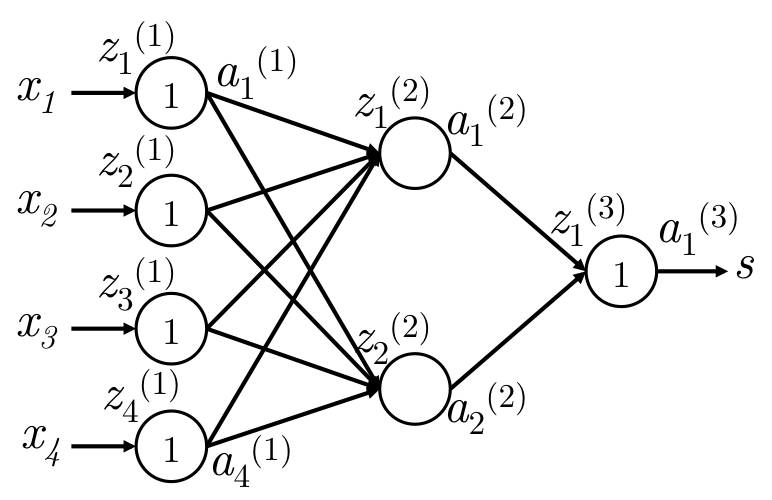
\includegraphics[width=0.5\textwidth]{images/eman/421nnet.png}%
     % you need to add the caption for the list of figures
\caption[Neural Network with several inputs and layers architecture ]{This is a 4-2-1 neural network where neuron $j$ on layer $k$ receives input $z_{j}^{(k)}$ and produces activation output $a_{j}^{(k)}$.}\label{fig:421nnet}%
  \end{figure}
Here, we use a neural network with a single hidden layer and a single unit output. Let us establish some \textbf{notation} that will make it easier to generalize this model later:
\begin{itemize}
\item $x_i$ is an input to the neural network.
\item $s$ is the output of the neural network.
\item Each layer (including the input and output layers) has neurons which receive an input and produce an output. The $j$-th neuron of layer $k$ receives the scalar input $z_j^{(k)}$ and produces the scalar activation output $a_j^{(k)}$.
\item We will call the backpropagated error calculated at $z_j^{(k)}$ as $\delta_j^{(k)}$.
\item Layer 1 refers to the input layer and not the first hidden layer. For the input layer, $x_j = z_j^{(1)} = a_j^{(1)}$.
\item $W^{(k)}$ is the transfer matrix that maps the output from the $k$-th layer to the input to the  $(k+1)$-th Thus, $W^{(1)} = W$ and $W^{(2)} = U$ to put this new generalized notation in perspective of Section~\ref{sec:ff}.
\end{itemize}
\textbf{Backpropagation Notation:}
\begin{itemize}
\item $x_i$ is an input to the neural network.
\item $s$ is the output of the neural network.
\item The $j$-th neuron of layer $k$ receives the scalar input $z_j^{(k)}$ and produces the scalar activation output $a_j^{(k)}$.
\item For the input layer, $x_j = z_j^{(1)} = a_j^{(1)}$.
\item $W^{(k)}$ is the transfer matrix that maps the output from the $k$-th layer to the input to the  $(k+1)$-th. Thus, $W^{(1)} = W$ and $W^{(2)} = U^T$ using notation from Section~\ref{sec:ff}.
\end{itemize}
\textbf{Let us begin:} Suppose the cost $J = (1 + s_c - s)$ is positive and we want to perform the update of parameter $W^{(1)}_{14}$ (in Figure~\ref{fig:421nnet} and Figure~\ref{fig:ErrorSignal}), we must realize that $W^{(1)}_{14}$ only contributes to $z_1^{(2)}$ and thus $a_1^{(2)}$. This fact is crucial to understanding backpropagation -- backpropagated gradients are only affected by values they contribute to. $a_1^{(2)}$ is consequently used in the forward computation of score by multiplication with $W^{(2)}_{1}$. We can see from the max-margin loss that:
$$\frac{\partial J}{\partial s} = - \frac{\partial J}{\partial s_c} =  -1$$
Therefore we will work with $\frac{\partial s}{\partial W^{(1)}_{ij}}$ here for simplicity. Thus,
\begin{align*}
\frac{\partial s}{\partial W^{(1)}_{ij}} &= \frac{\partial W^{(2)} a^{(2)}}{\partial W^{(1)}_{ij}} = \frac{\partial W^{(2)}_{i} a^{(2)}_i}{\partial W^{(1)}_{ij}} = W^{(2)}_{i} \frac{\partial a^{(2)}_i}{\partial W^{(1)}_{ij}}\\
\Rightarrow W^{(2)}_{i} \frac{\partial a^{(2)}_i}{\partial W^{(1)}_{ij}} &=  W^{(2)}_{i} \frac{\partial a^{(2)}_i}{\partial z^{(2)}_i} \frac{\partial z^{(2)}_i}{\partial W^{(1)}_{ij}}\\
&=  W^{(2)}_{i} \frac{f(z^{(2)}_i)}{\partial z^{(2)}_i} \frac{\partial z^{(2)}_i}{\partial W^{(1)}_{ij}}\\
&=  W^{(2)}_{i} f'(z^{(2)}_i) \frac{\partial z^{(2)}_i}{\partial W^{(1)}_{ij}}\\
&=  W^{(2)}_{i} f'(z^{(2)}_i) \frac{\partial}{\partial W^{(1)}_{ij}} (b^{(1)}_i + a_1^{(1)}  W^{(1)}_{i1} + a_2^{(1)}  W^{(1)}_{i2} + a_3^{(1)}  W^{(1)}_{i3} + a_4^{(1)}  W^{(1)}_{i4})\\
&=  W^{(2)}_{i} f'(z^{(2)}_i) \frac{\partial}{\partial W^{(1)}_{ij}} (b^{(1)}_i + \sum_k a_k^{(1)}  W^{(1)}_{ik})\\
&=  W^{(2)}_{i} f'(z^{(2)}_i) a_j^{(1)}\\
&=  \delta_i^{(2)} \cdot a_j^{(1)}
\end{align*}
We see above that the gradient reduces to the product $\delta_i^{(2)} \cdot a_j^{(1)}$ where $\delta_i^{(2)}$ is essentially the error propagating backwards from the $i$-th neuron in layer 2. $a_j^{(1)}$ is an input fed to $i$-th neuron in layer $2$ when scaled by $W_{ij}$.
\begin{figure}[H]%
    \center%
    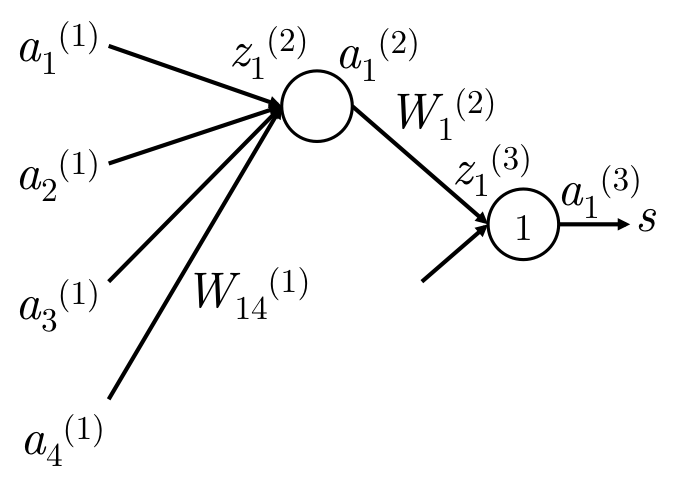
\includegraphics[width=0.5\textwidth]{images/eman/ErrorSignal.png}%
     % you need to add the caption for the list of figures
\caption[Subnetwork shows relevant parts of the network]{This subnetwork shows the relevant parts of the network required to update $W^{(1)}_{ij}$}\label{fig:ErrorSignal}%
  \end{figure}
Let us discuss the "error sharing/distribution" interpretation of backpropagation better using Figure~\ref{fig:ErrorSignal} as an example. Say we were to update $W^{(1)}_{14}$:

\begin{enumerate}
\item We start with the an error signal of 1 propagating backwards from $a_1^{(3)}$.
\item We then multiply this error by the local gradient of the neuron which maps $z_1^{(3)}$ to $a_1^{(3)}$. This happens to be $1$ in this case and thus, the error is still 1. This is now known as $\delta_1^{(3)} = 1$.
\item At this point, the error signal of 1 has reached $z_1^{(3)}$. We now need to distribute the error signal so that the "fair share" of the error reaches to $a_1^{(2)}$.
\item This amount is the (error signal at $z_1^{(3)} = \delta_1^{(3)}$)$ \times W_{1}^{(2)} = W_{1}^{(2)}$. Thus, the error at $a_1^{(2)} = W_{1}^{(2)}$.
\item As we did in step 2, we need to move the error across the neuron which maps $z_1^{(2)}$ to $a_1^{(2)}$. We do this by multiplying the error signal at $a_1^{(2)}$ by the local gradient of the neuron which happens to be $f'(z_1^{(2)})$.
\item Thus, the error signal at $z_1^{(2)}$ is $f'(z_1^{(2)})  W_{1}^{(2)}$. This is known as $\delta_1^{(2)}$.
\item Finally, we need to distribute the "fair share" of the error to $W^{(1)}_{14}$ by simply multiplying it by the input it was responsible for forwarding, which happens to be $a_4^{(1)}$.
\item Thus, the gradient of the loss with respect to $W^{(1)}_{14}$ is calculated to be $a_4^{(1)} f'(z_1^{(2)})  W_{1}^{(2)}$.
\end{enumerate}
Notice that the result we arrive at using this approach is exactly the same as that we arrived at using explicit differentiation earlier. Thus, we can calculate error gradients with respect to a parameter in the network using either the chain rule of differentiation or using an error sharing and distributed flow approach -- both of these approaches happen to do the exact same thing but it might be helpful to think about them one way or another.
$$ $$
\textbf{Bias Updates:} Bias terms (such as $b^{(1)}_1$) are mathematically equivalent to other weights contributing to the neuron input ($z^{(2)}_1$) as long as the input being forwarded is 1. As such, the bias gradients for neuron $i$ on layer $k$ is simply $\delta^{(k)}_i$. For instance, if we were updating $b_1^{(1)}$ instead of $W^{(1)}_{14}$ above, the gradient would simply be $f'(z_1^{(2)}) W_{1}^{(2)}$.
$$ $$
\textbf{Generalized steps to propagate $\delta^{(k)}$ to $\delta^{(k-1)}$:}
\begin{figure}[H]%
    \center%
    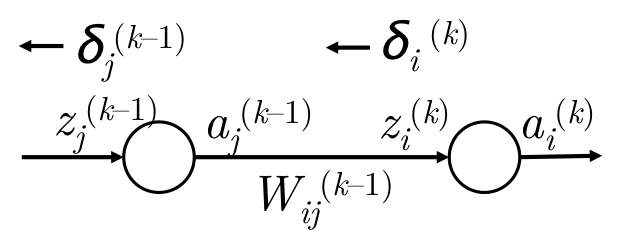
\includegraphics[width=0.5\textwidth]{images/eman/ErrorSignal2.png}%
     % you need to add the caption for the list of figures
\caption[Propagating error Neural Network]{Propagating error from $\delta^{(k)}$ to $\delta^{(k-1)}$}\label{fig:ErrorSignal2}%
  \end{figure}

\begin{enumerate}
\item We have error $\delta^{(k)}_i$ propagating backwards from $z^{(k)}_i$, i.e. neuron $i$ at layer $k$. See Figure~\ref{fig:ErrorSignal2}.
\item We propagate this error backwards to $a^{(k-1)}_j$ by multiplying $\delta^{(k)}_i$ by the path weight $W^{(k-1)}_{ij}$.
\item Thus, the error received at $a^{(k-1)}_j$ is $\delta^{(k)}_i W^{(k-1)}_{ij}$.
\item However, $a^{(k-1)}_j$ may have been forwarded to multiple nodes in the next layer as shown in Figure~\ref{fig:ErrorSignal3}. It should receive responsibility for errors propagating backward from node $m$ in layer $k$ too, using the exact same mechanism.
\item Thus, error received at $a^{(k-1)}_j$ is $\delta^{(k)}_i W^{(k-1)}_{ij} + \delta^{(k)}_m W^{(k-1)}_{mj}$.
\item In fact, we can generalize this to be $\sum_i \delta^{(k)}_i W^{(k-1)}_{ij}$.
\item Now that we have the correct error at $a^{(k-1)}_j$, we move it across neuron $j$ at layer $k-1$ by multiplying with with the local gradient $f'(z_j^{(k-1)})$.
\item Thus, the error that reaches $z_j^{(k-1)}$, called $\delta_j^{(k-1)}$ is \\$f'(z_j^{(k-1)}) \sum_i \delta^{(k)}_i W^{(k-1)}_{ij}$
\end{enumerate}

\begin{figure}[H]%
    \center%
    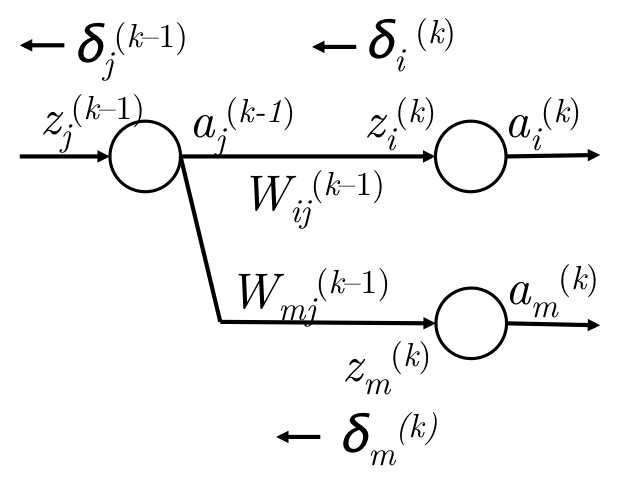
\includegraphics[width=0.5\textwidth]{images/eman/ErrorSignal3.png}%
     % you need to add the caption for the list of figures
\caption[Propagating error in Neural Network]{Propagating error from $\delta^{(k)}$ to $\delta^{(k-1)}$}\label{fig:ErrorSignal2}%
  \end{figure}
\subsection{Training with Backpropagation -- Vectorized}\label{sec:backprop2}

So far, we discussed how to calculate gradients for a given parameter in the model. Here we will generalize the approach above so that we update weight matrices and bias vectors all at once. Note that these are simply extensions of the above model that will help build intuition for the way error propagation can be done at a matrix-vector level.

For a given parameter $W_{ij}^{(k)}$, we identified that the error gradient is simply $\delta_{i}^{(k+1)}\cdot a_j^{(k)}$. As a reminder, $W^{(k)}$ is the matrix that maps $a^{(k)}$ to $z^{(k+1)}$. We can thus establish that the error gradient for the entire matrix $W^{(k)}$ is:
$$ \nabla_{W^{(k)}} = \begin{bmatrix} \delta_{1}^{(k+1)} a_1^{(k)} & \delta_{1}^{(k+1)} a_2^{(k)} & \cdots \\ \delta_{2}^{(k+1)} a_1^{(k)} & \delta_{2}^{(k+1)} a_2^{(k)} & \cdots \\ \vdots & \vdots & \ddots \end{bmatrix} = \delta^{(k+1)} a^{(k)T}$$

\textbf{Error propagates} from layer $(k+1)$ to $(k)$ in the following manner:
$$\delta^{(k)} = f'(z^{(k)}) \circ (W^{(k)T} \delta^{(k+1)})$$
Of course, this assumes that in the forward propagation the signal $z^{(k)}$ first goes through activation neurons $f$ to generate activations $a^{(k)}$ and are then linearly combined to yield $z^{(k+1)}$ via transfer matrix $W^{(k)}$.

Thus, we can write an entire matrix gradient using the outer product of the error vector propagating into the matrix and the activations forwarded by the matrix.

Now, we will see how we can calculate the error vector $\delta^{(k)}$. We established earlier using Figure~\ref{fig:ErrorSignal3} that $\delta^{(k)}_j =f'(z_j^{(k)}) \sum_i \delta^{(k+1)}_i W^{(k)}_{ij}$. This can easily generalize to matrices such that:
$$\delta^{(k)} = f'(z^{(k)}) \circ (W^{(k)T} \delta^{(k+1)}) $$
In the above formulation, the $\circ$ operator corresponds to an element wise product between elements of vectors ($\circ : \textbf{{R}}^N \times \textbf{{R}}^N \rightarrow \textbf{{R}}^N$).
$$ $$
\textbf{Computational efficiency:} Having explored element-wise updates as well as vector-wise updates, we must realize that the vectorized implementations run substantially faster in scientific computing environments such as MATLAB or Python (using NumPy/SciPy packages). Thus, we should use vectorized implementation in practice. Furthermore, we should also reduce redundant calculations in backpropagation - for instance, notice that $\delta^{(k)}$ depends directly on $\delta^{(k+1)}$. Thus, we should ensure that when we update $W^{(k)}$ using $\delta^{(k+1)}$, we save $\delta^{(k+1)}$ to later derive $\delta^{(k)}$ -- and we then repeat this for $(k-1)\hdots(1)$. Such a recursive procedure is what makes backpropagation a computationally affordable procedure.


